\chapter{Vyhodnocení detektorů stop v pevné fázi (praktická část)}
\section{Metodika}\label{sec:praktickaCast_metodika}
NPI používá materiál HARZLAS TD-1 (výrobce Nagase Landauer Ltd.) a od roku 2016 i TASTRAK (výrobce Track Analysis Systems Ltd.)~\cite{cesky}. HARZLAS TD-1 je leptán 18 hodin za teploty 70 $^{\circ}$C v 5 N koncentrovaném roztoku NaOH; odleptaná vrstva je kolem 15,3 $\mu$m. Velikost analyzované plochy se volí tak, aby bylo vyšetřeno alespoň tisíc stop (kvůli zajištění dostatečné statistiky). Detektor je tlustý 0.9 mm. TASTRAK se leptá dvoufázově: první fáze trvá 6 hodin a jsou při ní zobrazeny stopy vytvořené částicemi s velkým $\mathit{LET}$; při druhé fázi, která trvá dalších 9 hodin, se zobrazí i stopy pocházejících od částic s nižším $\mathit{LET}$. Celkový čas leptání je tedy 15 hodin. Buď se postupuje postupným leptáním (6 hodin leptání, vyhodnocení, 9 hodin leptání, vyhodnocení), nebo se část detektoru leptá 6 hodin a část 15 hodin, tudíž
detektor lze vyhodnotit najednou. Detektor se leptá při 70 $^{\circ}$C v 6,25 N koncentrovaném roztoku NaOH, odleptaná vrstva je tlustá 7,5/20,1 $\mu$m; velikost analyzované plochy TASTRAKu se volí stejným kritériem jako u HARZLAS TD-1. Po leptání následuje u obou detektorů nasnímání stop lineárním snímacím zařízením s vysokým rozlišením (které je součástí mikroskopu HSP-1000,~\cite{dosis_HSP1000}), poté jsou snímky se stopami analyzovány programem HspFit.

Zatímco HARZLAS TD-1 detekuje částice s $\LET$ vyšším než 7 keV/$\mu$m, TASTRAK má detekční práh 20 keV/$\mu$m~\cite{cesky,thesisKPBrabcova}. Na druhou stranu TASTRAK má vyšší rozsah měřitelných $\LET$ a díky leptání per partes detekuje s mnohem větší účinností částice s vyšším $\LET$ než HARZLAS TD-1~\cite{cesky}.
\newpage
%V tab. \ref{tab:praktickaCast_rozsahyLET} jsou rozsahy měřitelných $\LET$, tj. částice s $\LET$ v tomto intervalu můžeme zahrnout do výpočtů dávky, $\LET$ spektra atd.
%\begin{table}[H]
  %\centering
  %\caption{Rozsah měřitelných $\LET$ daného detektoru.~\cite{thesisKPBrabcova, cesky}}
  %\label{tab:praktickaCast_rozsahyLET}
  %\begin{tabular}{lll}
	%\toprule
	%Materiál & Rozsah $\LET$ [keV/$\mu$m]\\
	%\midrule
	%HARZLAS TD-1& 7 -- 340\\
	%TASTRAK& 20 -- 450\\
	%\bottomrule
  %\end{tabular}
%\end{table}
\section{Vyhodnocení}
\begin{wrapfigure}{r}{0.42\textwidth}
%\begin{figure}[h]
  \centering
  %\vspace{-20pt}
  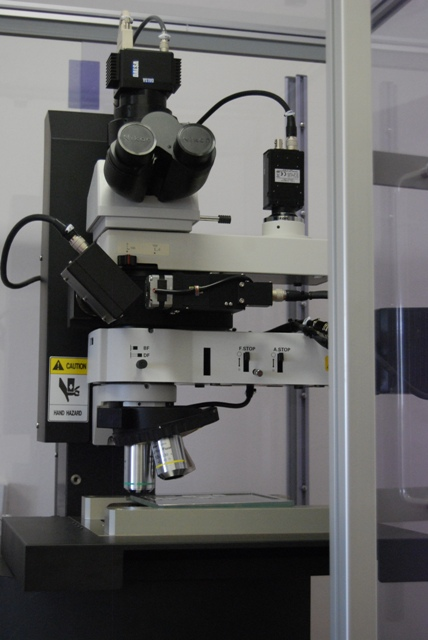
\includegraphics[width=0.4\textwidth]{praktickaCast_mikroskop}
  %\vspace{-20pt}
  \caption{Vysoko rychlostní optický mikroskop HSP-1000.~\cite{dosis_HSP1000}}
  \label{fig:praktickaCast_mikroskop}
  \vspace{-10pt}
%\end{figure}
\end{wrapfigure}
V praktické části bakalářské práce jsem vyhodnotil tři detektory stop osmé sady experimentu DOSIS3D. Detektory byly umístěny v prvním, druhém a třetím PDP. Jedná se o detektory z materiálu TASTRAK, které byly leptány 6 hodin, tj. zobrazené stopy jsou původem od částic s krátkým dosahem a vyšším LET.

Na obr.~\ref{fig:praktickaCast_mikroskop} je mikroskopický systém HSP-1000 (neúplný, chybí počítač, který systém řídí) pomocí něhož byl povrch detektorů nasnímán v dostatečném přiblížení.

Vyhodnocovat jsem započal analýzou stop v programu HspFit. Tento program sám vyhodnotí a zaznamená při dobrém nastavení určitých parametrů většinu stop, zbytek se musí označit ručně, což je zdlouhavá práce. Stopy se zaznamenávají tak, že se jejich okraj fituje elipsou, přičemž parametry fitu představují osy elipsy (hlavní $a$ a vedlejší $b$). V případě špatného automatického fitu lze proklad opravit ručně. Na obr.~\ref{fig:praktickaCast_hspfit} vidíme okno programu HspFit, zeleně jsou označeny stopy zaznamenané počítačem, fialově stopy zaznamenané uživatelem. Dále lze pozorovat, že některé stopy ještě zaznamenány nebyly. 
\begin{figure}[ht]
  \centering
  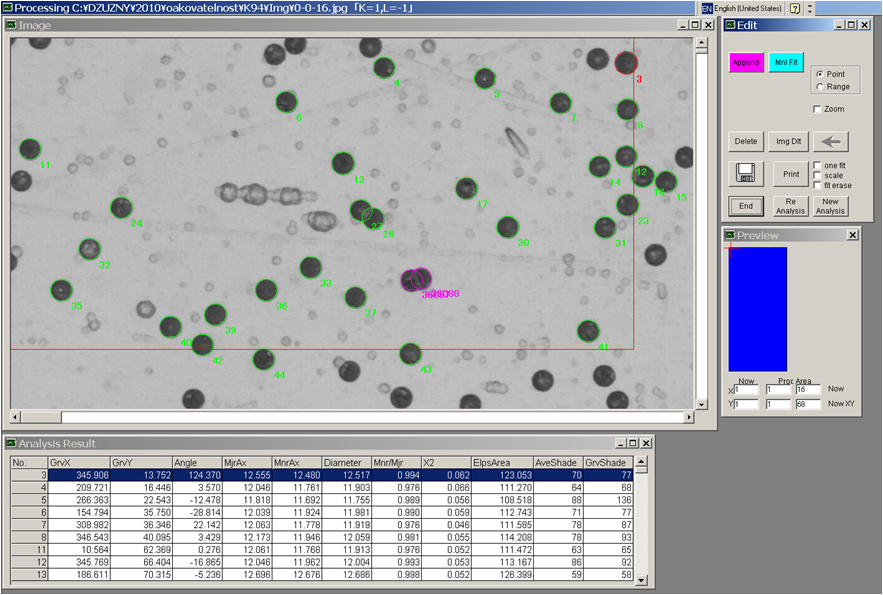
\includegraphics[width=0.85\textwidth]{praktickaCast_hspfit}
  \caption{Okno programu HspFit; zeleně jsou označeny fity vygenerované počítačem a fialově fity vytvořené uživatelem.~\cite{dosis_HSP1000}}
  \label{fig:praktickaCast_hspfit}
\end{figure}
\begin{figure}[p]
  \centering
  \begin{subfigure}{0.7\textwidth}
	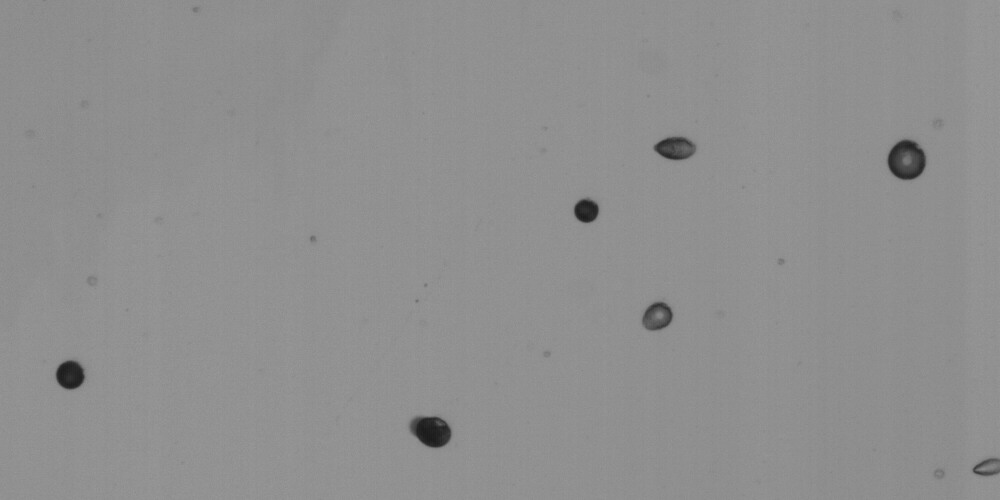
\includegraphics[width=\textwidth]{praktickaCast_stopyOK.jpg}
	\caption{}
  \end{subfigure}
  \begin{subfigure}{0.7\textwidth}
	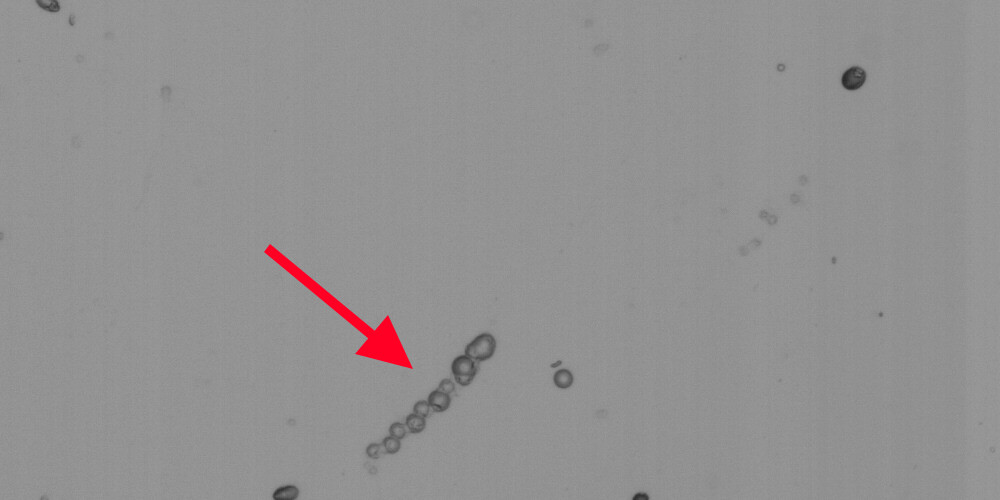
\includegraphics[width=\textwidth]{praktickaCast_stopyNeniStopa1.jpg}
	\caption{}
  \end{subfigure}
  \begin{subfigure}{0.7\textwidth}
	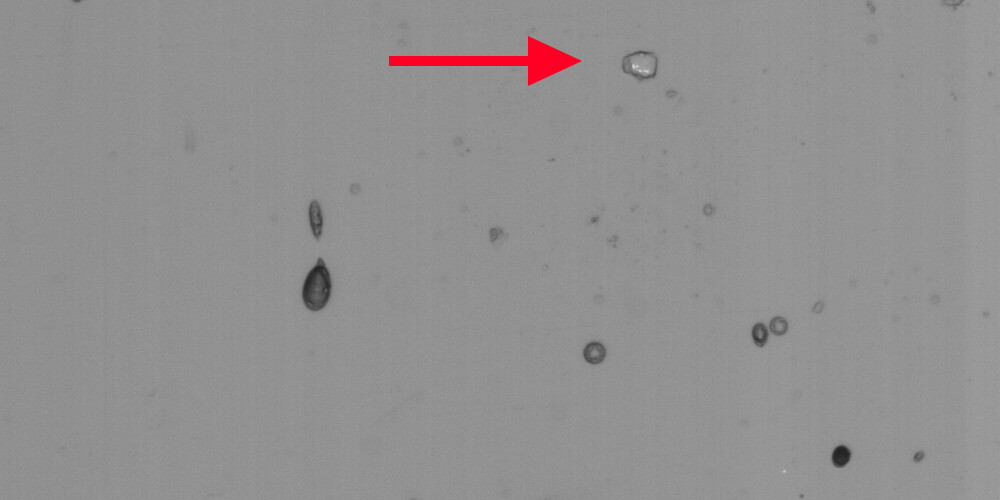
\includegraphics[width=\textwidth]{praktickaCast_stopyNeniStopa2.jpg}
	\caption{}
  \end{subfigure}
  \caption{Příklad naskenovaných snímků jednoho detektoru. V (a) jsou vidět normální stopy, v (b) a (c) naopak červené šipky ukazují na poškození materiálu, která nevznikla působením ionizujícího záření.}
  \label{fig:praktickaCast_stopy}
\end{figure}
\begin{figure}[ht]
  \centering
  \begin{subfigure}{0.7\textwidth}
	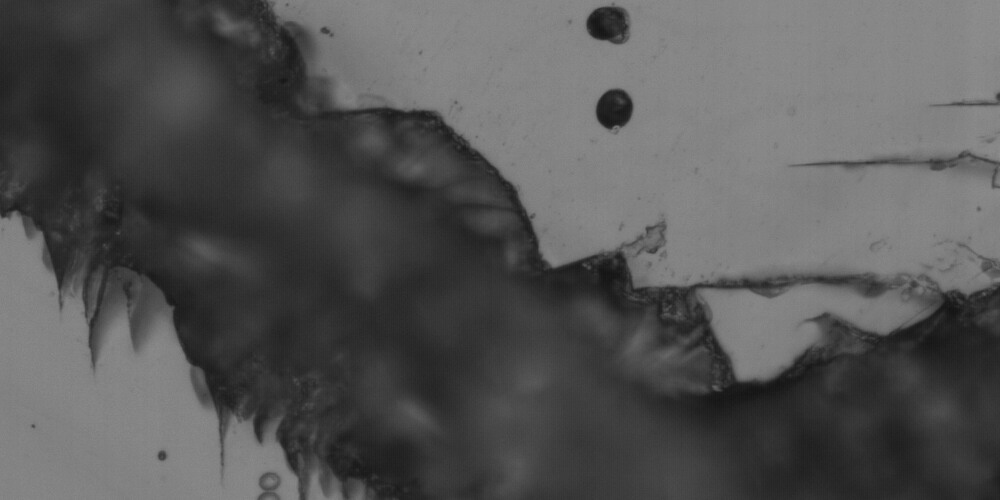
\includegraphics[width=\textwidth]{praktickaCast_stopyPoskozeni1.jpg}
	\caption{}
  \end{subfigure}
  \begin{subfigure}{0.7\textwidth}
	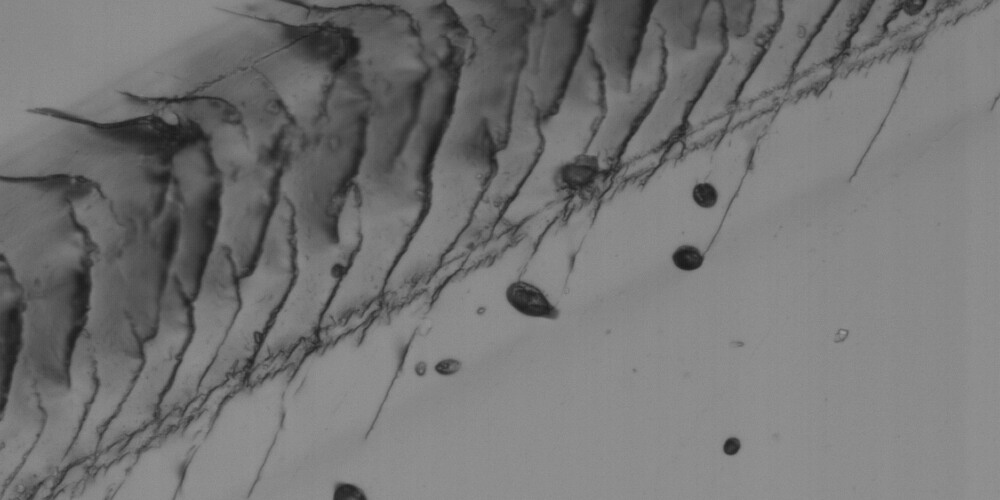
\includegraphics[width=\textwidth]{praktickaCast_stopyPoskozeni2.jpg}
	\caption{}
  \end{subfigure}
  \caption{Naskenované snímky zobrazující poškozené části plochy detektoru vyrytím křížků představující referenční body.}
  \label{fig:praktickaCast_stopyPoskozeni}
\end{figure}

V obr. \ref{fig:praktickaCast_stopy} jsou uvedeny jednotlivé snímky z povrchu náhodně vybraného detektoru. V (a) je snímek, který obsahuje čisté stopy; v (b) ukazuje červená šipka poškození materiálu nepocházející od ozáření ionizujícím zářením, které by mohl neznalý uživatel vyhodnotit jako vícero stop; v (c) taktéž ukazuje červená šipka poškození materiálu jiného charakteru. Obr.~\ref{fig:praktickaCast_stopyPoskozeni} pak ukazuje snímky, na nichž je naskenována plocha, která byla fyzicky znehodnocena člověkem vyrytím tří křížků. Ty představují referenční body. 

Osy všech elips byly spolu s dalšími parametry fitů (např. sklon elipsy) uloženy v souboru s příponou .nap. Tato data byla zpracována skriptem napsaném v programovacím jazyce Python, jehož výstupem jsou tři soubory. První soubor obsahuje údaje o poloze stopy, osách fitované elipsy, poměru leptacích rychlostí~$V$, korekčním součiniteli~$k_{\theta}$, lineárním přenosu energie~$\LET$, dávce a dávkovém ekvivalentu každé stopy. Druhý soubor obsahuje celkovou dávku a dávkový ekvivalent, které se absorbovaly v detektoru i s jejich příkony. Třetí soubor obsahuje data potřebná k vytvoření diferenciálních~$\LET$ spekter; z těchto dat jsem pomocí programu Gnuplot vytvořil~$\LET$ spektra (obr.~\ref{fig:praktickaCast_LETcetnost}, \ref{fig:praktickaCast_LETfluence},
\ref{fig:praktickaCast_LETdavka} a \ref{fig:praktickaCast_LETdavkEkvivalent}). Skript vypočítává pro každou částici $V$ z hodnot $a,b$ (vztah \eqref{eq:pomerLepRychlosti}, tloušťka odleptané vrstvy je $7,5$
$\mu$m) a následně~$\LET$ dané částice z $V$ pomocí kalibrační křivky pro TASTRAK leptaný 6 hodin
\begin{align}
  \LET(V) &= -99,8424+125,00172  V-15,28166  V^2+2,04636  V^3\,,\label{eq:kalibracniKrivkaSestHod}
  %\LET(V) &= -96,35071+114,90343  V-7,77194  V^2+1,27248  V^3\quad\text{(15 hod)},\label{eq:kalibracniKrivkaPatnactHod}
\end{align}
kde $\LET$ vychází v keV/$\mu$m; závislost byla přebrána z \cite{ssntd}. Kalibrační křivka je také k nahlédnutí na obr. \ref{fig:praktickaCast_kalibracniKrivky}. Kvůli jejímu rozsahu byly z dalšího vyhodnocování vyloučeny stopy s $\LET>1000$ keV/$\mu$.
\begin{figure}[ht]
  \centering
  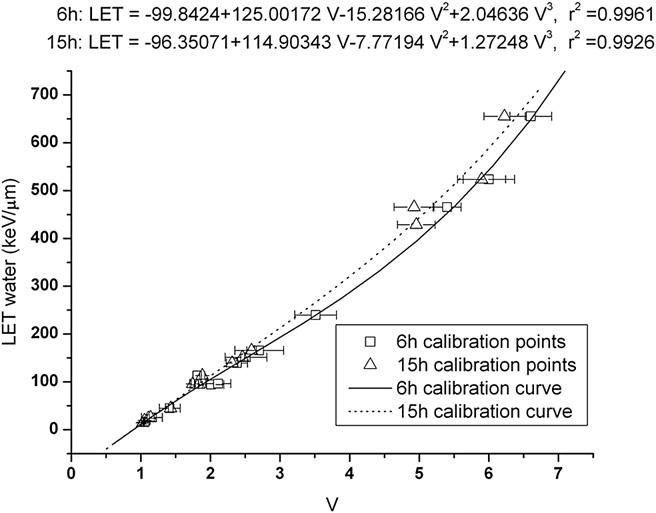
\includegraphics[width=0.7\textwidth]{praktickaCast_kalibracniKrivky.jpg}
  \caption{Kalibrační křivky pro TASTRAK leptaný 6, resp. 15 hodin. Obrázek obsahuje i kalibrační body. Kalibrační křivky pocházejí od MTA EK, \cite{ssntd}.}
  \label{fig:praktickaCast_kalibracniKrivky}
\end{figure}
Z $\LET$ všech částic jsou dále vypočítány dávka a dávkový ekvivalent dle vztahů \eqref{eq:Davka} a \eqref{eq:EkvDavka}. Díky známému času doby měření můžeme určit příkony těchto veličin, tj. $\dot{D}, \dot{H}$.

%Tab. \ref{tab:praktickaCast_davkyVysledky} obsahuje hledané celkové dávky a dávkové ekvivalenty; do vyhodnocení nebyly zahrnuty stopy s $\LET>1000$ (kvůli rozsahu kalibrační křivky). Na obr. \ref{fig:praktickaCast_LETspektra} jsou $\LET$ spektra získaná z vyhodnocených detektorů.

Původní Python skript, který jsem obdržel od vedoucí práce, neposkytoval data pro $\LET$ spektra a nevypočítával $\dot{D},\dot{H}$. Pro tyto účely jsem ho musel dopsat. 
 
V tab. \ref{tab:praktickaCast_analyzovanaPlocha} je velikost analyzované plochy a počet analyzovaných stop všech tří detektorů.
\begin{table}[H]
  \centering
  \caption{Velikost analyzované plochy a počet analyzovaných stop všech tří detektorů.}
  \label{tab:praktickaCast_analyzovanaPlocha}
  \begin{tabular}{lll}
	\toprule
	PDP&Analyzovaná plocha [mm$^2$]& Počet analyzovaných stop [-]\\
	\midrule
	1&13,35&1387\\
	2&14,03&1267\\
	3&13,66&1084\\
	\bottomrule
  \end{tabular}
\end{table}
\begin{table}[h]
  \centering
  \caption{Celkové dávky $D$, dávkové ekvivalenty $H$ a příkony $\dot{D},\dot{H}$ určené vyhodnocovanými detektory (doba měření=180 dní). $Q$ je průměrný jakostní faktor záření.}
  \label{tab:praktickaCast_davkyVysledky}
  \begin{tabular}{llllll}
	\toprule
	PDP&$D$ [mGy]&$H$ [mSv]&$\dot{D}$ [$\mu$Gy/den]&$\dot{H}$ [$\mu$Sv/den]& $Q$ [-]\\
	\midrule
	%1&5,31501450067&88,2754298605\\
	%2&5,068573344&92,5692674847\\
	%3&4,31129592097&75,4191405129\\
	1&$5\pm1$&$90\pm20$&$30\pm6$&$500\pm100$&$17\pm5$\\
	2&$5\pm1$&$90\pm20$&$28\pm6$&$500\pm100$&$18\pm5$\\
	3&$4\pm1$&$80\pm20$&$24\pm5$&$400\pm100$&$17\pm5$\\
	\bottomrule
  \end{tabular}
\end{table}

Tab. \ref{tab:praktickaCast_davkyVysledky} obsahuje hledané celkové dávky $D$ a dávkové ekvivalenty $H$ i s jejich příkony (detektory byly umístěny na pozicích 180 dní); do vyhodnocení nebyly zahrnuty stopy s $\LET>1000$ (kvůli rozsahu kalibrační křivky). Ze známosti $D$ a $H$ lze také určit kvalitu záření $Q=H/D$. Určení nepřesností je probráno dále v textu.

Na obrázcích \ref{fig:praktickaCast_LETcetnost}, \ref{fig:praktickaCast_LETfluence}, \ref{fig:praktickaCast_LETdavka} a \ref{fig:praktickaCast_LETdavkEkvivalent} jsou mnou vytvořená diferenciální $\LET$ spektra pro různé veličiny; $\LET$ intervaly byly zvoleny tak, aby byly na logaritmické ose ekvidistantní. První spektrum zobrazuje počet stop (detekovaných částic) spadnuvších do jednotlivých $\LET$ intervalů. Třetí, resp. čtvrté spektrum zobrazuje, jakou dávkou, resp. dávkovým ekvivalentem přispěly částice v daném $\LET$ intervalu do celkově obdržené dávky, resp. dávkového ekvivalentu. Druhé spektrum znázorňuje diferenciální fluenci $\Phi$ částic s $\LET$ v daném intervalu; $\Phi$ je definována vztahem
\begin{equation}
  \Phi=\frac{d^2N}{dAd\Omega}\,,
  \label{eq:praktickaCast_fluence}
\end{equation}
kde $dN$ je počet částic, které dopadly na kouli s příčným řezem o obsahu $dA$ pod prostorovým úhlem~$d\Omega$. K výpočtu $\Phi_i$ pro daný $\LET$ interval se používá vztah
\begin{equation}
  \Phi_i=\frac{N_i}{2\pi A\cos^2\theta_{k,i}}\,,
  \label{eq:praktickaCast_fluenceVypocet}
\end{equation}
kde $N_i$ je počet stop s $\LET$ v příslušném intervalu, $A$ je detekční plocha, $\cos^2\theta_{k,i}=\frac{V^2_i-1}{V^2_i}$ a $V_i$ je průměrná leptací rychlost uvažovaných stop \cite{ssntd}.

$\LET$ spektra jsou zatížena nepřesností, která pochází např. z nehomogenity materiálu detektoru a jeho tloušťky, rozdílů v koncentraci leptacího roztoku a v teplotách, nedokonalého smytí hydroxidu po leptání, výkonem vyhodnocovacího operátora~\cite{nejistoty}. Nechť $\Delta n$ je počet částic v jednom z $\LET$ intervalů. Lze uvažovat model \cite{nejistoty}, kdy nepřesnost určení $\Delta n$ pochází ze tří zdrojů:
\begin{itemize}
  \item nepřesnost $u_1(\Delta n)$ spojená s náhodností detekce částice, která má Poissonovo rozdělení, tj. $u_1=\sqrt{\Delta n}$;
  \item nepřesnost $u_2(\Delta n)$ vyplyvající z nepřesnosti kalibrační křivky, tj. závislosti $\LET(V)$;
  \item nepřesnost $u_3(\Delta n)$ spojená s odezvou detektoru.
\end{itemize}
Velikost $u_2$ jde zjistit pomocí známého vztahu pro výpočet nepřesností nepřímo měřených veličin
\begin{equation}
  u^2(f)=\left(\frac{\partial f}{\partial x}u(x)\right)^2+\left( \frac{\partial f}{\partial y}u(y) \right)^2+2\frac{\partial f}{\partial x}\frac{\partial f}{\partial y}u(x,y)\,,
  \label{eq:praktickaCast_neprimaChyba}
\end{equation}
který je pro zjednodušení uveden pro funkci $f$ závislou pouze na dvou veličinách $x,y$, obecně jich může být více; $u(x), u(y)$ jsou chyby veličin $x,y$; $u(x,y)$ je jejich kovariance. Tedy pro $u_2$
\begin{equation}
  u_2(\Delta n)\approx\frac{\Delta n}{\Delta\LET}u(\LET)\,,
  \label{eq:praktickaCast_u2}
\end{equation}
kde $\Delta\LET$ je délka uvažovaného intervalu a $u(\LET)$ je nepřesnost určení lineárního přenosu energie z kalibrační křivky, která se zjistí také použitím vztahu \eqref{eq:praktickaCast_neprimaChyba} pro $\LET(V)$; diferenciály jsou z důvodu jednoduchosti a praktičnosti aproximovány na $\Delta n, \Delta\LET$. Poměr leptacích rychlostí závisí na $a,b,d$, tzn. na osách elipsy (stopy) a tloušťce odleptané vrstvy. Chyba $V$ se určí zase podle vztahu \eqref{eq:praktickaCast_neprimaChyba} pro $V(a,b,d)$. Kovariance $u(a,d)$ a $u(b,d)$ jsou brány jako nulové, jelikož se nedají snadno určit; vzhledem k zápornosti příslušných parciálních derivací tímto krokem $u(V)$ nadhodnocujeme. Určení $u(a), u(b), u(a,b), u(d)$ spolu s tzv. očekávanými hodnotami $a,b,d$ je podrobně
rozebráno v~\cite{nejistoty}.

Třetí složka nejistot $u_3$ se dá určit jen v některých situacích, viz~\cite{nejistoty}.

Chyba určení dávky $D_i$ od $N_i$ částic s lineárním přenosem energie $\LET_i$ se zjistí aplikací vztahu \eqref{eq:praktickaCast_neprimaChyba} pro $D_i(\LET_i,N_i)$, tedy 
\begin{equation}
  u(D_i)=\sqrt{\left(\frac{\partial D_i}{\partial\LET_i}u(\LET_i)\right)^2+\left(\frac{\partial D_i}{\partial N_i}u(N_i)\right)^2}\,,
  \label{eq:praktickaCast_chybaDavka}
\end{equation}
kde vzhledem k Poissonovu rozdělení náhodné veličiny $N_i$ je $u(N_i)=\sqrt{N_i}$,~\cite{thesisKPBrabcova}; $u(\LET_i)$ se určí způsobem popsaným výše. Nepřesnost dávkového ekvivalentu se zjistí obdobně.

Do $\LET$ spekter jsem nepřesnosti nezahrnul. Relativní chyba $D$ a $H$ je zhruba 20~\%~\cite{nejistoty}.
\begin{figure}[H]
  \centering
	\centering
	% GNUPLOT: LaTeX picture with Postscript
\begingroup
  \makeatletter
  \providecommand\color[2][]{%
    \GenericError{(gnuplot) \space\space\space\@spaces}{%
      Package color not loaded in conjunction with
      terminal option `colourtext'%
    }{See the gnuplot documentation for explanation.%
    }{Either use 'blacktext' in gnuplot or load the package
      color.sty in LaTeX.}%
    \renewcommand\color[2][]{}%
  }%
  \providecommand\includegraphics[2][]{%
    \GenericError{(gnuplot) \space\space\space\@spaces}{%
      Package graphicx or graphics not loaded%
    }{See the gnuplot documentation for explanation.%
    }{The gnuplot epslatex terminal needs graphicx.sty or graphics.sty.}%
    \renewcommand\includegraphics[2][]{}%
  }%
  \providecommand\rotatebox[2]{#2}%
  \@ifundefined{ifGPcolor}{%
    \newif\ifGPcolor
    \GPcolortrue
  }{}%
  \@ifundefined{ifGPblacktext}{%
    \newif\ifGPblacktext
    \GPblacktexttrue
  }{}%
  % define a \g@addto@macro without @ in the name:
  \let\gplgaddtomacro\g@addto@macro
  % define empty templates for all commands taking text:
  \gdef\gplbacktext{}%
  \gdef\gplfronttext{}%
  \makeatother
  \ifGPblacktext
    % no textcolor at all
    \def\colorrgb#1{}%
    \def\colorgray#1{}%
  \else
    % gray or color?
    \ifGPcolor
      \def\colorrgb#1{\color[rgb]{#1}}%
      \def\colorgray#1{\color[gray]{#1}}%
      \expandafter\def\csname LTw\endcsname{\color{white}}%
      \expandafter\def\csname LTb\endcsname{\color{black}}%
      \expandafter\def\csname LTa\endcsname{\color{black}}%
      \expandafter\def\csname LT0\endcsname{\color[rgb]{1,0,0}}%
      \expandafter\def\csname LT1\endcsname{\color[rgb]{0,1,0}}%
      \expandafter\def\csname LT2\endcsname{\color[rgb]{0,0,1}}%
      \expandafter\def\csname LT3\endcsname{\color[rgb]{1,0,1}}%
      \expandafter\def\csname LT4\endcsname{\color[rgb]{0,1,1}}%
      \expandafter\def\csname LT5\endcsname{\color[rgb]{1,1,0}}%
      \expandafter\def\csname LT6\endcsname{\color[rgb]{0,0,0}}%
      \expandafter\def\csname LT7\endcsname{\color[rgb]{1,0.3,0}}%
      \expandafter\def\csname LT8\endcsname{\color[rgb]{0.5,0.5,0.5}}%
    \else
      % gray
      \def\colorrgb#1{\color{black}}%
      \def\colorgray#1{\color[gray]{#1}}%
      \expandafter\def\csname LTw\endcsname{\color{white}}%
      \expandafter\def\csname LTb\endcsname{\color{black}}%
      \expandafter\def\csname LTa\endcsname{\color{black}}%
      \expandafter\def\csname LT0\endcsname{\color{black}}%
      \expandafter\def\csname LT1\endcsname{\color{black}}%
      \expandafter\def\csname LT2\endcsname{\color{black}}%
      \expandafter\def\csname LT3\endcsname{\color{black}}%
      \expandafter\def\csname LT4\endcsname{\color{black}}%
      \expandafter\def\csname LT5\endcsname{\color{black}}%
      \expandafter\def\csname LT6\endcsname{\color{black}}%
      \expandafter\def\csname LT7\endcsname{\color{black}}%
      \expandafter\def\csname LT8\endcsname{\color{black}}%
    \fi
  \fi
    \setlength{\unitlength}{0.0500bp}%
    \ifx\gptboxheight\undefined%
      \newlength{\gptboxheight}%
      \newlength{\gptboxwidth}%
      \newsavebox{\gptboxtext}%
    \fi%
    \setlength{\fboxrule}{0.5pt}%
    \setlength{\fboxsep}{1pt}%
\begin{picture}(7936.00,5102.00)%
    \gplgaddtomacro\gplbacktext{%
      \csname LTb\endcsname%
      \put(946,704){\makebox(0,0)[r]{\strut{}$1$}}%
      \csname LTb\endcsname%
      \put(946,2082){\makebox(0,0)[r]{\strut{}$10$}}%
      \csname LTb\endcsname%
      \put(946,3459){\makebox(0,0)[r]{\strut{}$100$}}%
      \csname LTb\endcsname%
      \put(946,4837){\makebox(0,0)[r]{\strut{}$1000$}}%
      \csname LTb\endcsname%
      \put(1078,484){\makebox(0,0){\strut{}$10$}}%
      \csname LTb\endcsname%
      \put(4309,484){\makebox(0,0){\strut{}$100$}}%
      \csname LTb\endcsname%
      \put(7539,484){\makebox(0,0){\strut{}$1000$}}%
    }%
    \gplgaddtomacro\gplfronttext{%
      \csname LTb\endcsname%
      \put(176,2770){\rotatebox{-270}{\makebox(0,0){\strut{}$N$ [-]}}}%
      \put(4308,154){\makebox(0,0){\strut{}$\mathit{LET}$ [keV/$\mu$m]}}%
      \csname LTb\endcsname%
      \put(6624,4616){\makebox(0,0)[r]{\strut{}PDP1}}%
      \csname LTb\endcsname%
      \put(6624,4301){\makebox(0,0)[r]{\strut{}PDP2}}%
      \csname LTb\endcsname%
      \put(6624,3986){\makebox(0,0)[r]{\strut{}PDP3}}%
    }%
    \gplbacktext
    \put(0,0){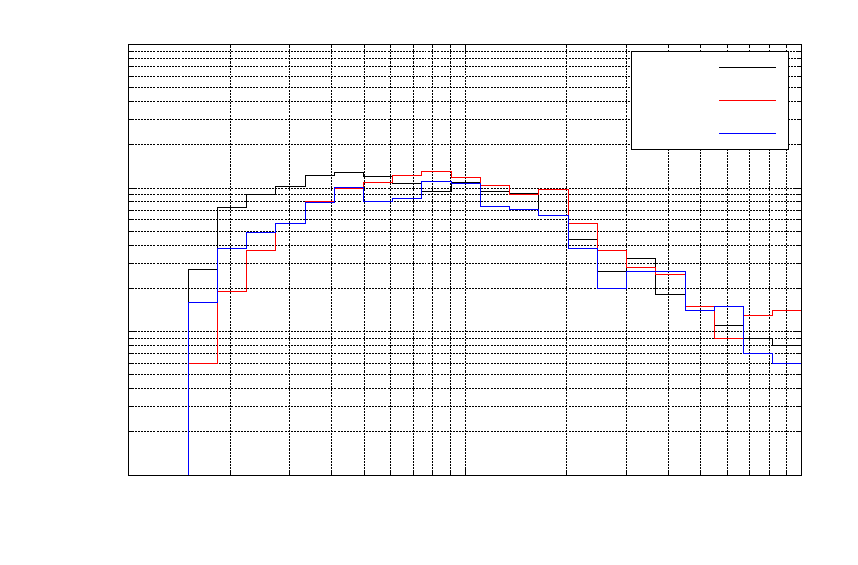
\includegraphics{LETspektrumCetnost}}%
    \gplfronttext
  \end{picture}%
\endgroup

	\caption{$\LET$ spektra vyhodnocených detektorů, na vertikální ose je počet stop v intervalu.}
	\label{fig:praktickaCast_LETcetnost}
\end{figure}
\begin{figure}[H]
  \centering
	\centering
	% GNUPLOT: LaTeX picture with Postscript
\begingroup
  \makeatletter
  \providecommand\color[2][]{%
    \GenericError{(gnuplot) \space\space\space\@spaces}{%
      Package color not loaded in conjunction with
      terminal option `colourtext'%
    }{See the gnuplot documentation for explanation.%
    }{Either use 'blacktext' in gnuplot or load the package
      color.sty in LaTeX.}%
    \renewcommand\color[2][]{}%
  }%
  \providecommand\includegraphics[2][]{%
    \GenericError{(gnuplot) \space\space\space\@spaces}{%
      Package graphicx or graphics not loaded%
    }{See the gnuplot documentation for explanation.%
    }{The gnuplot epslatex terminal needs graphicx.sty or graphics.sty.}%
    \renewcommand\includegraphics[2][]{}%
  }%
  \providecommand\rotatebox[2]{#2}%
  \@ifundefined{ifGPcolor}{%
    \newif\ifGPcolor
    \GPcolortrue
  }{}%
  \@ifundefined{ifGPblacktext}{%
    \newif\ifGPblacktext
    \GPblacktexttrue
  }{}%
  % define a \g@addto@macro without @ in the name:
  \let\gplgaddtomacro\g@addto@macro
  % define empty templates for all commands taking text:
  \gdef\gplbacktext{}%
  \gdef\gplfronttext{}%
  \makeatother
  \ifGPblacktext
    % no textcolor at all
    \def\colorrgb#1{}%
    \def\colorgray#1{}%
  \else
    % gray or color?
    \ifGPcolor
      \def\colorrgb#1{\color[rgb]{#1}}%
      \def\colorgray#1{\color[gray]{#1}}%
      \expandafter\def\csname LTw\endcsname{\color{white}}%
      \expandafter\def\csname LTb\endcsname{\color{black}}%
      \expandafter\def\csname LTa\endcsname{\color{black}}%
      \expandafter\def\csname LT0\endcsname{\color[rgb]{1,0,0}}%
      \expandafter\def\csname LT1\endcsname{\color[rgb]{0,1,0}}%
      \expandafter\def\csname LT2\endcsname{\color[rgb]{0,0,1}}%
      \expandafter\def\csname LT3\endcsname{\color[rgb]{1,0,1}}%
      \expandafter\def\csname LT4\endcsname{\color[rgb]{0,1,1}}%
      \expandafter\def\csname LT5\endcsname{\color[rgb]{1,1,0}}%
      \expandafter\def\csname LT6\endcsname{\color[rgb]{0,0,0}}%
      \expandafter\def\csname LT7\endcsname{\color[rgb]{1,0.3,0}}%
      \expandafter\def\csname LT8\endcsname{\color[rgb]{0.5,0.5,0.5}}%
    \else
      % gray
      \def\colorrgb#1{\color{black}}%
      \def\colorgray#1{\color[gray]{#1}}%
      \expandafter\def\csname LTw\endcsname{\color{white}}%
      \expandafter\def\csname LTb\endcsname{\color{black}}%
      \expandafter\def\csname LTa\endcsname{\color{black}}%
      \expandafter\def\csname LT0\endcsname{\color{black}}%
      \expandafter\def\csname LT1\endcsname{\color{black}}%
      \expandafter\def\csname LT2\endcsname{\color{black}}%
      \expandafter\def\csname LT3\endcsname{\color{black}}%
      \expandafter\def\csname LT4\endcsname{\color{black}}%
      \expandafter\def\csname LT5\endcsname{\color{black}}%
      \expandafter\def\csname LT6\endcsname{\color{black}}%
      \expandafter\def\csname LT7\endcsname{\color{black}}%
      \expandafter\def\csname LT8\endcsname{\color{black}}%
    \fi
  \fi
    \setlength{\unitlength}{0.0500bp}%
    \ifx\gptboxheight\undefined%
      \newlength{\gptboxheight}%
      \newlength{\gptboxwidth}%
      \newsavebox{\gptboxtext}%
    \fi%
    \setlength{\fboxrule}{0.5pt}%
    \setlength{\fboxsep}{1pt}%
\begin{picture}(7936.00,5102.00)%
    \gplgaddtomacro\gplbacktext{%
      \csname LTb\endcsname%
      \put(946,704){\makebox(0,0)[r]{\strut{}$1$}}%
      \csname LTb\endcsname%
      \put(946,2082){\makebox(0,0)[r]{\strut{}$10$}}%
      \csname LTb\endcsname%
      \put(946,3459){\makebox(0,0)[r]{\strut{}$100$}}%
      \csname LTb\endcsname%
      \put(946,4837){\makebox(0,0)[r]{\strut{}$1000$}}%
      \csname LTb\endcsname%
      \put(1078,484){\makebox(0,0){\strut{}$10$}}%
      \csname LTb\endcsname%
      \put(4309,484){\makebox(0,0){\strut{}$100$}}%
      \csname LTb\endcsname%
      \put(7539,484){\makebox(0,0){\strut{}$1000$}}%
    }%
    \gplgaddtomacro\gplfronttext{%
      \csname LTb\endcsname%
      \put(176,2770){\rotatebox{-270}{\makebox(0,0){\strut{}$\Phi$ [cm$^{-2}$sr$^{-1}$]}}}%
      \put(4308,154){\makebox(0,0){\strut{}$\mathit{LET}$ [keV/$\mu$m]}}%
      \csname LTb\endcsname%
      \put(6624,4616){\makebox(0,0)[r]{\strut{}PDP1}}%
      \csname LTb\endcsname%
      \put(6624,4301){\makebox(0,0)[r]{\strut{}PDP2}}%
      \csname LTb\endcsname%
      \put(6624,3986){\makebox(0,0)[r]{\strut{}PDP3}}%
    }%
    \gplbacktext
    \put(0,0){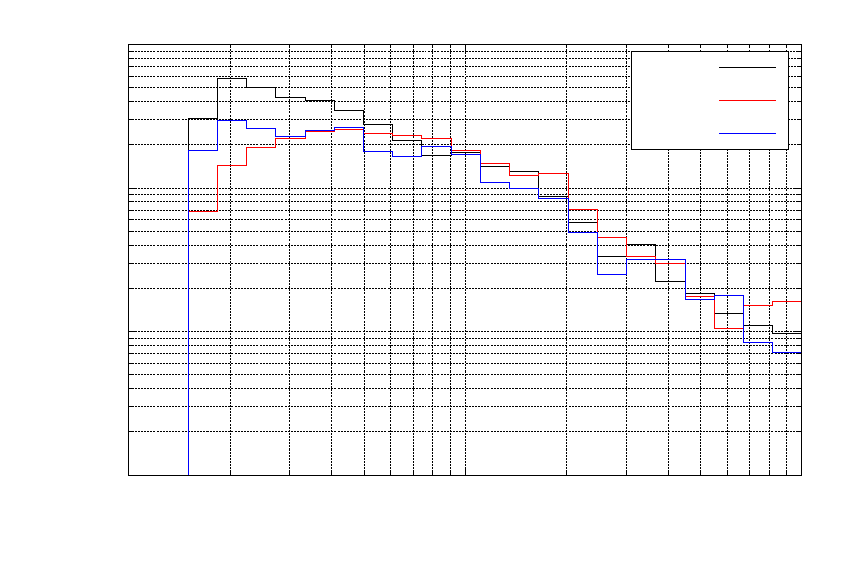
\includegraphics{LETspektrumFluence}}%
    \gplfronttext
  \end{picture}%
\endgroup

	\caption{$\LET$ spektra detektorů pro fluenci.}
	\label{fig:praktickaCast_LETfluence}
\end{figure}
\begin{figure}[H]
  \centering
	\centering
	% GNUPLOT: LaTeX picture with Postscript
\begingroup
  \makeatletter
  \providecommand\color[2][]{%
    \GenericError{(gnuplot) \space\space\space\@spaces}{%
      Package color not loaded in conjunction with
      terminal option `colourtext'%
    }{See the gnuplot documentation for explanation.%
    }{Either use 'blacktext' in gnuplot or load the package
      color.sty in LaTeX.}%
    \renewcommand\color[2][]{}%
  }%
  \providecommand\includegraphics[2][]{%
    \GenericError{(gnuplot) \space\space\space\@spaces}{%
      Package graphicx or graphics not loaded%
    }{See the gnuplot documentation for explanation.%
    }{The gnuplot epslatex terminal needs graphicx.sty or graphics.sty.}%
    \renewcommand\includegraphics[2][]{}%
  }%
  \providecommand\rotatebox[2]{#2}%
  \@ifundefined{ifGPcolor}{%
    \newif\ifGPcolor
    \GPcolortrue
  }{}%
  \@ifundefined{ifGPblacktext}{%
    \newif\ifGPblacktext
    \GPblacktexttrue
  }{}%
  % define a \g@addto@macro without @ in the name:
  \let\gplgaddtomacro\g@addto@macro
  % define empty templates for all commands taking text:
  \gdef\gplbacktext{}%
  \gdef\gplfronttext{}%
  \makeatother
  \ifGPblacktext
    % no textcolor at all
    \def\colorrgb#1{}%
    \def\colorgray#1{}%
  \else
    % gray or color?
    \ifGPcolor
      \def\colorrgb#1{\color[rgb]{#1}}%
      \def\colorgray#1{\color[gray]{#1}}%
      \expandafter\def\csname LTw\endcsname{\color{white}}%
      \expandafter\def\csname LTb\endcsname{\color{black}}%
      \expandafter\def\csname LTa\endcsname{\color{black}}%
      \expandafter\def\csname LT0\endcsname{\color[rgb]{1,0,0}}%
      \expandafter\def\csname LT1\endcsname{\color[rgb]{0,1,0}}%
      \expandafter\def\csname LT2\endcsname{\color[rgb]{0,0,1}}%
      \expandafter\def\csname LT3\endcsname{\color[rgb]{1,0,1}}%
      \expandafter\def\csname LT4\endcsname{\color[rgb]{0,1,1}}%
      \expandafter\def\csname LT5\endcsname{\color[rgb]{1,1,0}}%
      \expandafter\def\csname LT6\endcsname{\color[rgb]{0,0,0}}%
      \expandafter\def\csname LT7\endcsname{\color[rgb]{1,0.3,0}}%
      \expandafter\def\csname LT8\endcsname{\color[rgb]{0.5,0.5,0.5}}%
    \else
      % gray
      \def\colorrgb#1{\color{black}}%
      \def\colorgray#1{\color[gray]{#1}}%
      \expandafter\def\csname LTw\endcsname{\color{white}}%
      \expandafter\def\csname LTb\endcsname{\color{black}}%
      \expandafter\def\csname LTa\endcsname{\color{black}}%
      \expandafter\def\csname LT0\endcsname{\color{black}}%
      \expandafter\def\csname LT1\endcsname{\color{black}}%
      \expandafter\def\csname LT2\endcsname{\color{black}}%
      \expandafter\def\csname LT3\endcsname{\color{black}}%
      \expandafter\def\csname LT4\endcsname{\color{black}}%
      \expandafter\def\csname LT5\endcsname{\color{black}}%
      \expandafter\def\csname LT6\endcsname{\color{black}}%
      \expandafter\def\csname LT7\endcsname{\color{black}}%
      \expandafter\def\csname LT8\endcsname{\color{black}}%
    \fi
  \fi
    \setlength{\unitlength}{0.0500bp}%
    \ifx\gptboxheight\undefined%
      \newlength{\gptboxheight}%
      \newlength{\gptboxwidth}%
      \newsavebox{\gptboxtext}%
    \fi%
    \setlength{\fboxrule}{0.5pt}%
    \setlength{\fboxsep}{1pt}%
\begin{picture}(7936.00,5102.00)%
    \gplgaddtomacro\gplbacktext{%
      \csname LTb\endcsname%
      \put(946,704){\makebox(0,0)[r]{\strut{}$10$}}%
      \csname LTb\endcsname%
      \put(946,2771){\makebox(0,0)[r]{\strut{}$100$}}%
      \csname LTb\endcsname%
      \put(946,4837){\makebox(0,0)[r]{\strut{}$1000$}}%
      \csname LTb\endcsname%
      \put(1078,484){\makebox(0,0){\strut{}$10$}}%
      \csname LTb\endcsname%
      \put(4309,484){\makebox(0,0){\strut{}$100$}}%
      \csname LTb\endcsname%
      \put(7539,484){\makebox(0,0){\strut{}$1000$}}%
    }%
    \gplgaddtomacro\gplfronttext{%
      \csname LTb\endcsname%
      \put(176,2770){\rotatebox{-270}{\makebox(0,0){\strut{}$D$ [$\mu$Gy]}}}%
      \put(4308,154){\makebox(0,0){\strut{}$\mathit{LET}$ [keV/$\mu$m]}}%
      \csname LTb\endcsname%
      \put(6624,4616){\makebox(0,0)[r]{\strut{}PDP1}}%
      \csname LTb\endcsname%
      \put(6624,4301){\makebox(0,0)[r]{\strut{}PDP2}}%
      \csname LTb\endcsname%
      \put(6624,3986){\makebox(0,0)[r]{\strut{}PDP3}}%
    }%
    \gplbacktext
    \put(0,0){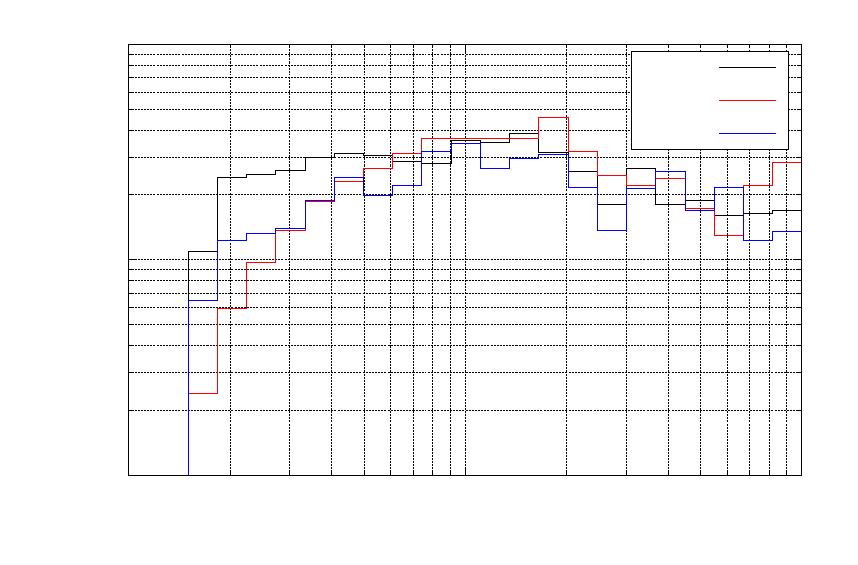
\includegraphics{LETspektrumDavka}}%
    \gplfronttext
  \end{picture}%
\endgroup

	\caption{$\LET$ spektra detektorů pro dávku.}
	\label{fig:praktickaCast_LETdavka}
\end{figure}
\begin{figure}[H]
  \centering
	\centering
	% GNUPLOT: LaTeX picture with Postscript
\begingroup
  \makeatletter
  \providecommand\color[2][]{%
    \GenericError{(gnuplot) \space\space\space\@spaces}{%
      Package color not loaded in conjunction with
      terminal option `colourtext'%
    }{See the gnuplot documentation for explanation.%
    }{Either use 'blacktext' in gnuplot or load the package
      color.sty in LaTeX.}%
    \renewcommand\color[2][]{}%
  }%
  \providecommand\includegraphics[2][]{%
    \GenericError{(gnuplot) \space\space\space\@spaces}{%
      Package graphicx or graphics not loaded%
    }{See the gnuplot documentation for explanation.%
    }{The gnuplot epslatex terminal needs graphicx.sty or graphics.sty.}%
    \renewcommand\includegraphics[2][]{}%
  }%
  \providecommand\rotatebox[2]{#2}%
  \@ifundefined{ifGPcolor}{%
    \newif\ifGPcolor
    \GPcolortrue
  }{}%
  \@ifundefined{ifGPblacktext}{%
    \newif\ifGPblacktext
    \GPblacktexttrue
  }{}%
  % define a \g@addto@macro without @ in the name:
  \let\gplgaddtomacro\g@addto@macro
  % define empty templates for all commands taking text:
  \gdef\gplbacktext{}%
  \gdef\gplfronttext{}%
  \makeatother
  \ifGPblacktext
    % no textcolor at all
    \def\colorrgb#1{}%
    \def\colorgray#1{}%
  \else
    % gray or color?
    \ifGPcolor
      \def\colorrgb#1{\color[rgb]{#1}}%
      \def\colorgray#1{\color[gray]{#1}}%
      \expandafter\def\csname LTw\endcsname{\color{white}}%
      \expandafter\def\csname LTb\endcsname{\color{black}}%
      \expandafter\def\csname LTa\endcsname{\color{black}}%
      \expandafter\def\csname LT0\endcsname{\color[rgb]{1,0,0}}%
      \expandafter\def\csname LT1\endcsname{\color[rgb]{0,1,0}}%
      \expandafter\def\csname LT2\endcsname{\color[rgb]{0,0,1}}%
      \expandafter\def\csname LT3\endcsname{\color[rgb]{1,0,1}}%
      \expandafter\def\csname LT4\endcsname{\color[rgb]{0,1,1}}%
      \expandafter\def\csname LT5\endcsname{\color[rgb]{1,1,0}}%
      \expandafter\def\csname LT6\endcsname{\color[rgb]{0,0,0}}%
      \expandafter\def\csname LT7\endcsname{\color[rgb]{1,0.3,0}}%
      \expandafter\def\csname LT8\endcsname{\color[rgb]{0.5,0.5,0.5}}%
    \else
      % gray
      \def\colorrgb#1{\color{black}}%
      \def\colorgray#1{\color[gray]{#1}}%
      \expandafter\def\csname LTw\endcsname{\color{white}}%
      \expandafter\def\csname LTb\endcsname{\color{black}}%
      \expandafter\def\csname LTa\endcsname{\color{black}}%
      \expandafter\def\csname LT0\endcsname{\color{black}}%
      \expandafter\def\csname LT1\endcsname{\color{black}}%
      \expandafter\def\csname LT2\endcsname{\color{black}}%
      \expandafter\def\csname LT3\endcsname{\color{black}}%
      \expandafter\def\csname LT4\endcsname{\color{black}}%
      \expandafter\def\csname LT5\endcsname{\color{black}}%
      \expandafter\def\csname LT6\endcsname{\color{black}}%
      \expandafter\def\csname LT7\endcsname{\color{black}}%
      \expandafter\def\csname LT8\endcsname{\color{black}}%
    \fi
  \fi
    \setlength{\unitlength}{0.0500bp}%
    \ifx\gptboxheight\undefined%
      \newlength{\gptboxheight}%
      \newlength{\gptboxwidth}%
      \newsavebox{\gptboxtext}%
    \fi%
    \setlength{\fboxrule}{0.5pt}%
    \setlength{\fboxsep}{1pt}%
\begin{picture}(7936.00,5102.00)%
    \gplgaddtomacro\gplbacktext{%
      \csname LTb\endcsname%
      \put(1210,704){\makebox(0,0)[r]{\strut{}$10$}}%
      \csname LTb\endcsname%
      \put(1210,1737){\makebox(0,0)[r]{\strut{}$100$}}%
      \csname LTb\endcsname%
      \put(1210,2771){\makebox(0,0)[r]{\strut{}$1000$}}%
      \csname LTb\endcsname%
      \put(1210,3804){\makebox(0,0)[r]{\strut{}$10000$}}%
      \csname LTb\endcsname%
      \put(1210,4837){\makebox(0,0)[r]{\strut{}$100000$}}%
      \csname LTb\endcsname%
      \put(1342,484){\makebox(0,0){\strut{}$10$}}%
      \csname LTb\endcsname%
      \put(4441,484){\makebox(0,0){\strut{}$100$}}%
      \csname LTb\endcsname%
      \put(7539,484){\makebox(0,0){\strut{}$1000$}}%
    }%
    \gplgaddtomacro\gplfronttext{%
      \csname LTb\endcsname%
      \put(176,2770){\rotatebox{-270}{\makebox(0,0){\strut{}$H$ [$\mu$Sv]}}}%
      \put(4440,154){\makebox(0,0){\strut{}$\mathit{LET}$ [keV/$\mu$m]}}%
      \csname LTb\endcsname%
      \put(6624,4616){\makebox(0,0)[r]{\strut{}PDP1}}%
      \csname LTb\endcsname%
      \put(6624,4301){\makebox(0,0)[r]{\strut{}PDP2}}%
      \csname LTb\endcsname%
      \put(6624,3986){\makebox(0,0)[r]{\strut{}PDP3}}%
    }%
    \gplbacktext
    \put(0,0){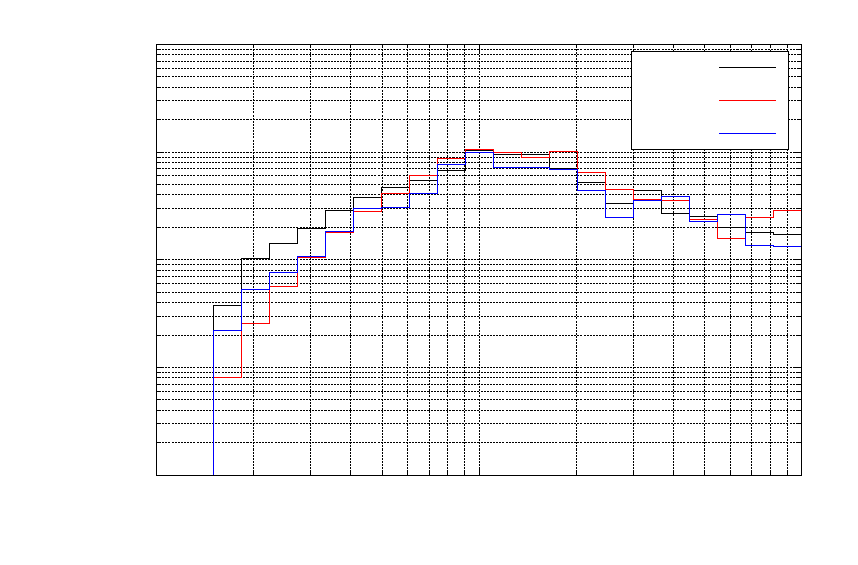
\includegraphics{LETspektrumDavkEkvivalent}}%
    \gplfronttext
  \end{picture}%
\endgroup

	\caption{$\LET$ spektra detektorů pro dávkový ekvivalent.}
	\label{fig:praktickaCast_LETdavkEkvivalent}
\end{figure}
\newpage
\section{Diskuze}
Ze spekter vidíme, že byly registrovány částice s $\LET\in[15;1000]$ keV/$\mu$m; dolní hranice je dána detekčním prahem TASTRAKu a horní hranice byla uměle nastavena s přihlédnutím k rozsahu kalibrační křivky. Nejpočetnější složku tvoří dle spektra~\ref{fig:praktickaCast_LETcetnost} stopy s $\LET$ v rozsahu 30 až 200 keV/$\mu$m. Ty odpovídají nejspíš protonům, které pocházejí z SAA nebo z interakcí neutronů s materiálem detektoru, a $\alpha$ částicím. Protony mají v CR-39 maximální $\LET$ kolem 80-90~keV/$\mu$m, $\alpha$ částice kolem 200~keV/$\mu$m~\cite{SRIM}. Stopy s nižším $\LET$ odpovídají iontům z primárního kosmického záření, stopy s vyšším $\LET$ odraženým jádrům O, C atd. Ze stejného spektra je také vidět, že bylo detekováno relativně málo částic s malým $\LET$ (mezi 20 a 30
keV/$\mu$m). To je způsobeno kratší dobou leptání detektorů, po které nebyla většina stop s malým $\LET$ ještě odhalena. 

Na obr. \ref{fig:praktickaCast_LETcetnost} a v tab. \ref{tab:praktickaCast_analyzovanaPlocha} je vidět, že v prvním detektoru bylo analyzováno nejvíce stop a že tento nadbytek oproti ostatním detektorům tvoří stopy s nižším $\LET$. Toto může být způsobeno tím, že jsem při ručním analyzování stop prvního detektoru připustil do dalších výpočtů i tzv. přeleptané stopy. To jsou stopy od částic s krátkým dosahem (sekundárních částic), pro které byla doba leptání příliš dlouhá, takže započalo jejich odstraňování, ale ne tak ne tak dlouhá, aby byly odstraněny úplně. Přeleptané stopy neposkytují žádnou relevantní informaci.

Spektra pro dávku a dávkový příkon názorně ukazují rozdíl mezi těmito dvěma veličinami. Tab.~\ref{tab:praktickaCast_relPrispevkyDavka} zobrazuje relativní příspěvky k $D$ a $H$ od částic s různým $\LET$.
\begin{table}[ht]
  \centering
  \caption{Relativní příspěvky zaokrouhlené na jednotky k celkové dávce $D$, resp. k celkovému dávkovému ekvivalentu $H$ od částic z daného $\LET$ intervalu.}
  \label{tab:praktickaCast_relPrispevkyDavka}
  \begin{tabular}{lll}
	\toprule
	$\LET$ [keV/$\mu$m]& $D_{\text{rel}}$ [-]&$H_{\text{rel}}$ [-]\\
	\midrule
	$[22;33]$&9 \%&3 \%\\
	$[110;200]$&20 \%&28 \%\\
	$[546;812]$&8 \%&5 \%\\
	\bottomrule
  \end{tabular}
\end{table}

Dávkové příkony určené z vyhodnocených TED (tab.~\ref{tab:praktickaCast_davkyVysledky}) jsou mnohem menší než dávkové příkony určené z TLD (viz. oddíl \ref{sec:dosis_vysledky}; lze předpokládat, že $\dot{D}$ z osmé sady budou vycházet alespoň řádově jako $\dot{D}$ v předchozích sadách). Je to tím, že převážná část absorbované dávky pochází od částic s $\LET$ menším než je detekční práh TASTRAKu. Tento rozdíl dávkových příkonů od TLD a TED byl naměřen i v jiných experimentech, např.~\cite{passDetectors,ambrozova_dvaExperimenty, japonsky}.

Vyhodnocování bude pokračovat druhým leptáním, při kterém se zobrazí částice s menším $\LET$ delším dosahem. Bude leptána stejná plocha a díky referenčním bodům (obr.~\ref{fig:praktickaCast_stopyPoskozeni}) bude možné rozlišit jednotlivé stopy od sekundárních a primárních částic. Stopy od sekundárních částic, které byly zřetelné po prvním leptání, budou nyní odleptány, případně přeleptány, a naopak se zobrazí předtím neviděné stopy od primárních částic, které mají dlouhý dosah. Vypočtou se dávky a dávkové ekvivalenty nových stop a poté se připočtou k $D$ a $H$ určené už při prvním leptání. Nakonec se kombinací dat z TLD a TED postupem popsaným v oddíle~\ref{sec:detektory_kombinace} určí celkové dávkové příkony a dávkové ekvivalenty.
